\documentclass{standalone}
  \usepackage{tikz}
  \usetikzlibrary{arrows.meta, automata, bending, positioning, shapes.misc}
  \tikzstyle{automaton}=[shorten >=1pt, >={Stealth[bend,round]}, initial text=]

\begin{document}
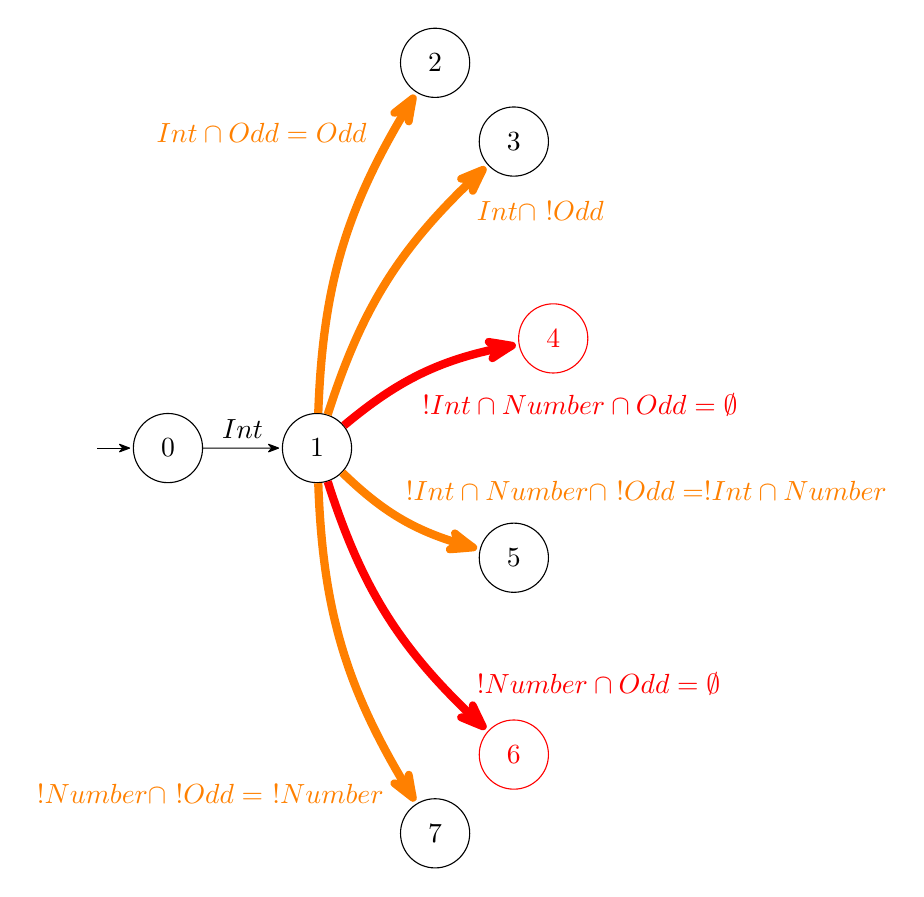
\begin{tikzpicture}[automaton, auto]
  \node[state,initial,rounded rectangle] (0) {$0$};
  \node[state,rounded rectangle] (1) [right=10mm of 0] {$1$};
  \node[state,rounded rectangle] (2) [above right=40mm and 15mm of 1] {$2$};
  \node[state,rounded rectangle] (3) [above right=30mm and 25mm of 1] {$3$};
  \node[state,color=red,rounded rectangle] (4) [above right=5mm and 30mm of 1] {$4$};
  \node[state,rounded rectangle] (5) [below right=5mm and 25mm of 1] {$5$};
  \node[state,color=red,rounded rectangle] (6) [below right=30mm and 25mm of 1] {$6$};
  \node[state,rounded rectangle] (7) [below right=40mm and 15mm of 1] {$7$};
  \path[->] (0) edge node {$Int$} (1);
  \path[->] (1) edge[orange, line width=3pt, bend left=15]  node[pos=.8] {$Int \cap Odd = Odd$} (2);
  \path[->] (1) edge[orange, line width=3pt, bend left=15]  node[pos=.9,swap] {$Int \cap ~!Odd $} (3);
  \path[->] (1) edge[red, line width=3pt, bend left=15]  node[pos=.4,swap] {$!Int \cap Number\cap Odd = \emptyset$} (4);
  \path[->] (1) edge[orange, line width=3pt, bend right=15]  node[pos=.4] {$!Int \cap Number\cap~ !Odd = !Int \cap Number$} (5);
  \path[->] (1) edge[red, line width=3pt, bend right=15] node[pos=.9] {$!Number\cap Odd = \emptyset$} (6);
  \path[->] (1) edge[orange, line width=3pt, bend right=15] node[swap,pos=.9] {$!Number\cap ~!Odd = ~!Number$} (7);
\end{tikzpicture}
\end{document}
